% ==============================================================================
% cover.tex — Academic Book Cover Architecture (3D Pixar Semi-realistics & TikZ)
% Standards: academic-book-cover-architect (Aspect Ratio 2:3, Full-Bleed 6x9 in)
% ==============================================================================
\begin{titlepage}
\thispagestyle{empty}

\begingroup
\setlength{\XeTeXlinebreakskip}{0pt}

\begin{tikzpicture}[remember picture, overlay]
    % 1. Full-Bleed High-Resolution Artwork (figures/cover_art.jpg)
    \node[anchor=center, inner sep=0pt] at (current page.center) {
        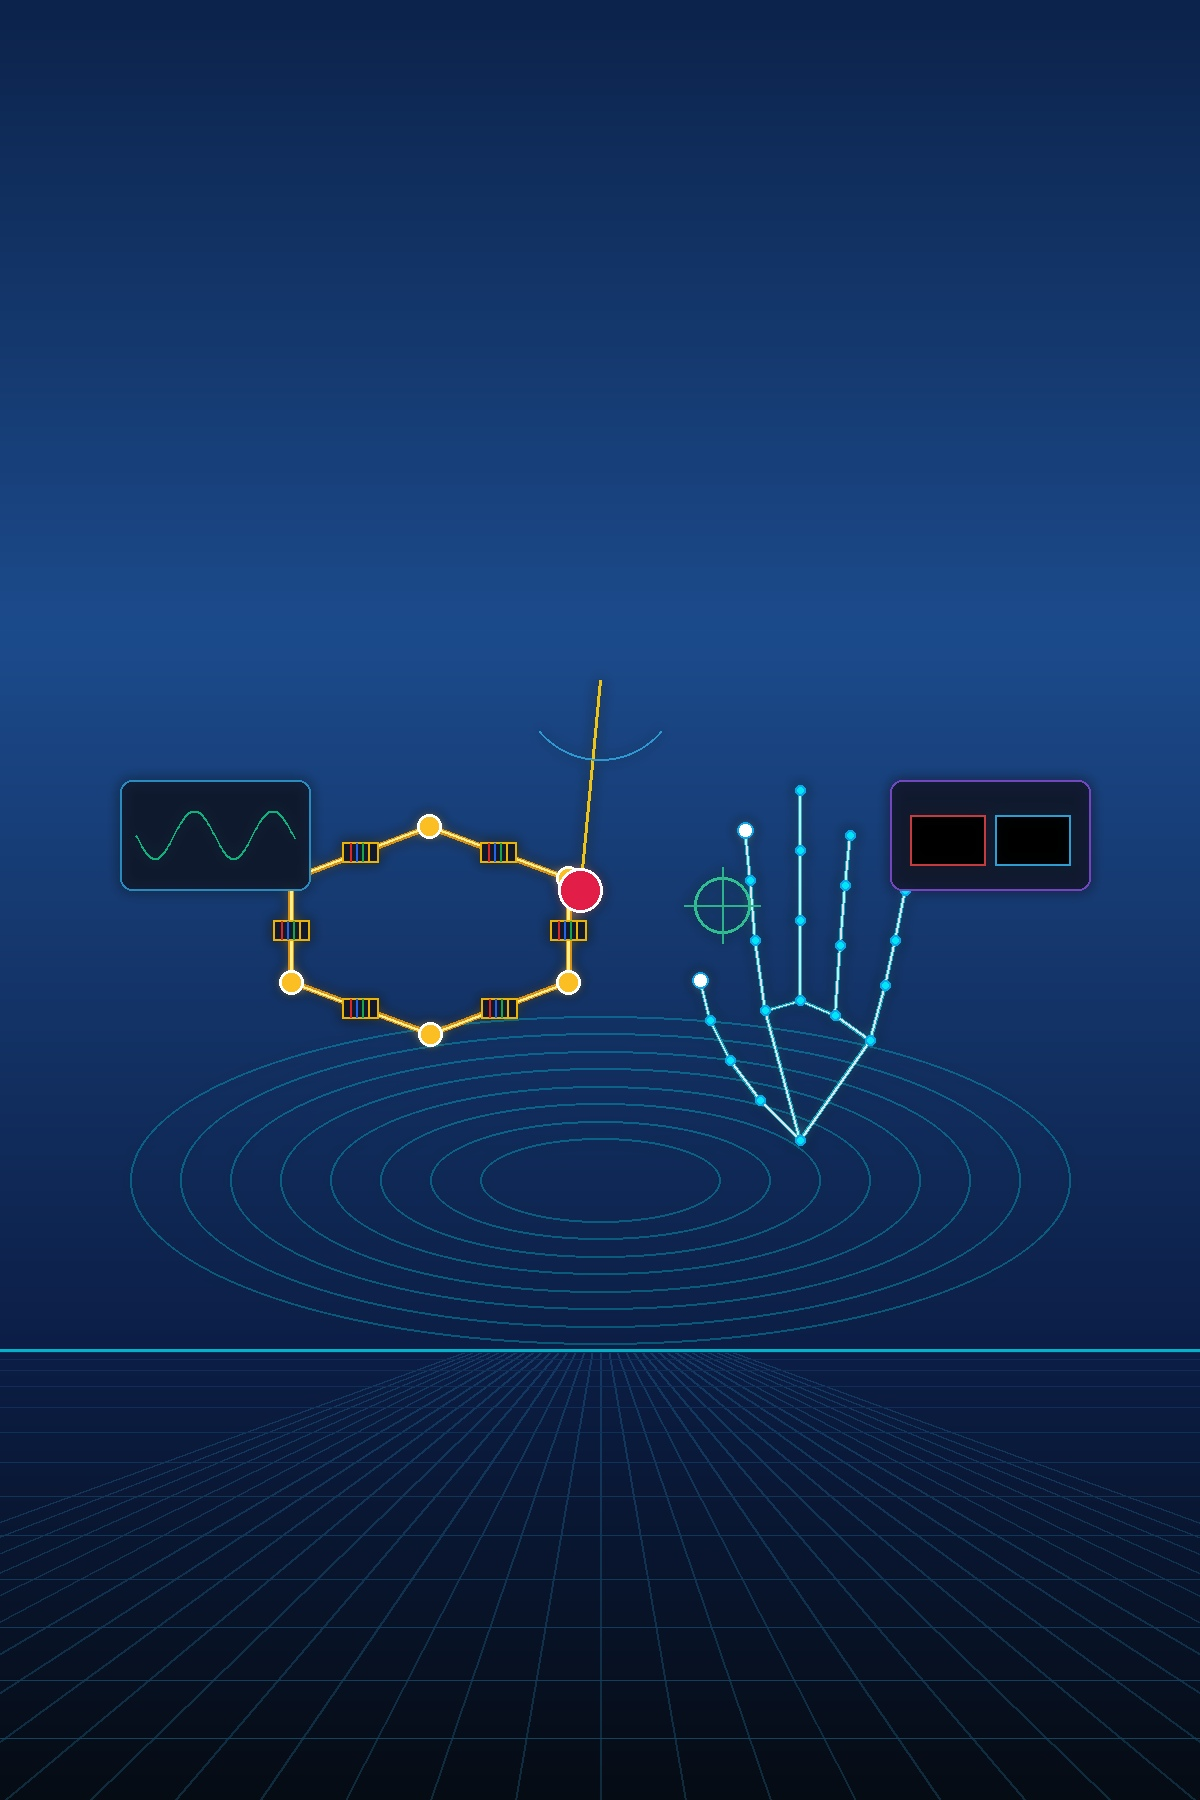
\includegraphics[width=\paperwidth,height=\paperheight]{figures/cover_art.jpg}
    };

    % --------------------------------------------------------------------------
    % 2. UPPER SKY ZONE: DUAL-LAYER MICRO DROP-SHADOW
    % --------------------------------------------------------------------------
    % 2.1 Category Badge
    \node[anchor=north, align=center, text width=5.2in] 
          at ([yshift=-0.42in]current page.north) {
        {\fontsize{8.5}{11}\selectfont\bfseries\color{white}%
        \colorbox{rbruBlue!70!black}{\quad HANDS-ON WORKSHOP HANDBOOK \textbullet\ คู่มือการอบรมเชิงปฏิบัติการ \quad}}
    };

    % 2.2 Main Title Line 1 & Line 2 (Layer 1: Deep Black Micro Drop-Shadow)
    \node[anchor=north, align=center, text width=5.6in] 
          at ([xshift=0.7pt, yshift=-0.76in]current page.north) {
        {\fontsize{16.5}{21}\selectfont\bfseries\color{black} การออกแบบและพัฒนาสื่อการสอนสามมิติเสมือนจริง}\\[6pt]
        {\fontsize{17.5}{23}\selectfont\bfseries\color{black} และความจริงเสริมด้วยปัญญาประดิษฐ์}
    };

    % 2.3 Main Title Line 1 & Line 2 (Layer 2: Crisp Pure White & Cyan Neon)
    \node[anchor=north, align=center, text width=5.6in] 
          at ([yshift=-0.75in]current page.north) {
        {\fontsize{16.5}{21}\selectfont\bfseries\color{white} การออกแบบและพัฒนาสื่อการสอนสามมิติเสมือนจริง}\\[6pt]
        {\fontsize{17.5}{23}\selectfont\bfseries\color{cyan!90!white} และความจริงเสริมด้วยปัญญาประดิษฐ์}
    };

    % 2.4 English Subtitle
    \node[anchor=north, align=center, text width=5.6in] 
          at ([yshift=-2.02in]current page.north) {
        {\fontsize{7.5}{9.5}\selectfont\bfseries\color{rbruGold!95!white}%
        DESIGNING \& DEVELOPING 3D VIRTUAL \& AUGMENTED REALITY INSTRUCTIONAL MEDIA WITH AI}
    };

    % --------------------------------------------------------------------------
    % 3. LOWER GROUND ZONE: DUAL-LAYER MICRO DROP-SHADOW (LIGHT TEXT ON DARK GROUND)
    % --------------------------------------------------------------------------
    % 3.1 Author & Affiliation Metadata (Layer 1: Deep Black Drop Shadow)
    \node[anchor=south, align=center, text width=5.4in] 
          at ([xshift=0.6pt, yshift=0.34in]current page.south) {
        {\fontsize{13}{16}\selectfont\bfseries\color{black} ผู้ช่วยศาสตราจารย์ ดร.ชีวะ ทัศนา}\\[3pt]
        {\fontsize{8.5}{11}\selectfont\color{black} ศูนย์ความเป็นเลิศด้านสิ่งแวดล้อมและพลังงาน (LEQs) คณะวิทยาศาสตร์และเทคโนโลยี}\\[4pt]
        {\fontsize{8}{10}\selectfont\color{black} มหาวิทยาลัยราชภัฏรำไพพรรณี \textbullet\ พ.ศ. 2569}
    };

    % 3.2 Author & Affiliation Metadata (Layer 2: Crisp Pure White & Warm Gold)
    \node[anchor=south, align=center, text width=5.4in] 
          at ([yshift=0.35in]current page.south) {
        {\fontsize{13}{16}\selectfont\bfseries\color{white} ผู้ช่วยศาสตราจารย์ ดร.ชีวะ ทัศนา}\\[3pt]
        {\fontsize{8.5}{11}\selectfont\color{white!95} ศูนย์ความเป็นเลิศด้านสิ่งแวดล้อมและพลังงาน (LEQs) คณะวิทยาศาสตร์และเทคโนโลยี}\\[4pt]
        {\fontsize{8}{10}\selectfont\color{yellow!90!white} มหาวิทยาลัยราชภัฏรำไพพรรณี \textbullet\ พ.ศ. 2569}
    };

\end{tikzpicture}

\endgroup
\end{titlepage}
\clearpage
\thispagestyle{empty}
\null\clearpage
